\documentclass{beamer}
\usepackage{graphicx}
% \usepackage{wrapfig}
\usepackage{setspace}
\usepackage{xcolor}
\usetheme{Madrid}
\usecolortheme{default}

\title[22MP0D48]{Block chain and Cryptography Communication System}
\subtitle{Project ID:22MP0D48\\}
\author[Review -II]{Group~Members RA1811003030185~Koustubh Saxena RA1811003030202 Satwik Srivastava  RA1811003030204 Rachit Gupta RA1811003030302~Deeptanshu Yadav  {Supervised By Dr. Premananda Sahu}}
\institute[]{Department of Computer Science \& Engineerin Faculty of Engineering \& Technolog SRM Institute of Science \& Technology}
\logo{
\includegraphics[scale=.4]{srm_logo}}
\date{\today}

\begin{document}
	\begin{frame}
		\maketitle
		\date{}
	\end{frame}
	\begin{frame}[allowframebreaks]{Table of Contents}
		\tableofcontents[sections={1-7}]
		\tableofcontents[sections={8-10}]
	\end{frame}
	
	\begin{frame}{Comments}
		\LARGE
		\begin{itemize}
			\item Make your Objectives concise and to the point.
			\item Make your PPT more discriptive.
			\item Use LateX to create presentation, and use the template provided
			\medskip
		\end{itemize}
	\end{frame}
	\begin{frame}{Action Taken}
		\begin{itemize}
			\LARGE
			\item Defined a precise obective and made the objective clear.
			\item Added more slides.
			\item Used the template provided.
		\end{itemize}
	\end{frame}

	\section{Objectives \& Motivation}
	\begin{frame}{Objectives \& Motivation}
		\LARGE
	A prototype of fast and secure communication of the data over the internet is achieved by using military grade encryption followed by passing the data using Blockchain technology	
	\end{frame}

	\section{Literature Survey}
	\begin{frame}{Literature Survey}
	\bigskip
	\normalsize
		\begin{itemize}
			\item A systematic review of blockchain-based applications across multiple domains.
			\medskip
			\item We identify the characteristics that can revolutionise "business-as-usual" practices.
			\medskip
			\item We provide a framework to determine the fitness of blockchainn per application.
			\medskip
			\item  To evaluate feassibility of blockchain application in real-time envoirments. 
		\end{itemize}
	\end{frame}
	
	\section{Architectural Design of the Proposed System}
	\begin{frame}{Blockchain}
	\bigskip
	\normalsize
	A blockchain is essentially a digital ledger of transactions that is duplicated and distributed across the entire network of computer systems on the blackchains. Each block in the chain contains a number of transactions, and every time a new transactions occurs on the blockchain, a record of that transaction is added to every participant's ledger. 
	\end{frame}

	\begin{frame}{BLOCKS}
	\bigskip
	\normalsize
	What Is a Block (Blockchain Block)? Blocks are \textbf(data structures within the blockchain database, where transaction data in a cryptocurrency blockchain are permanently record.) A block records some or all of the most recent transactions not yet validated by the network. Once the data are validated, the block is closed.
	\end{frame}

	\begin{frame}{Blockchain}
	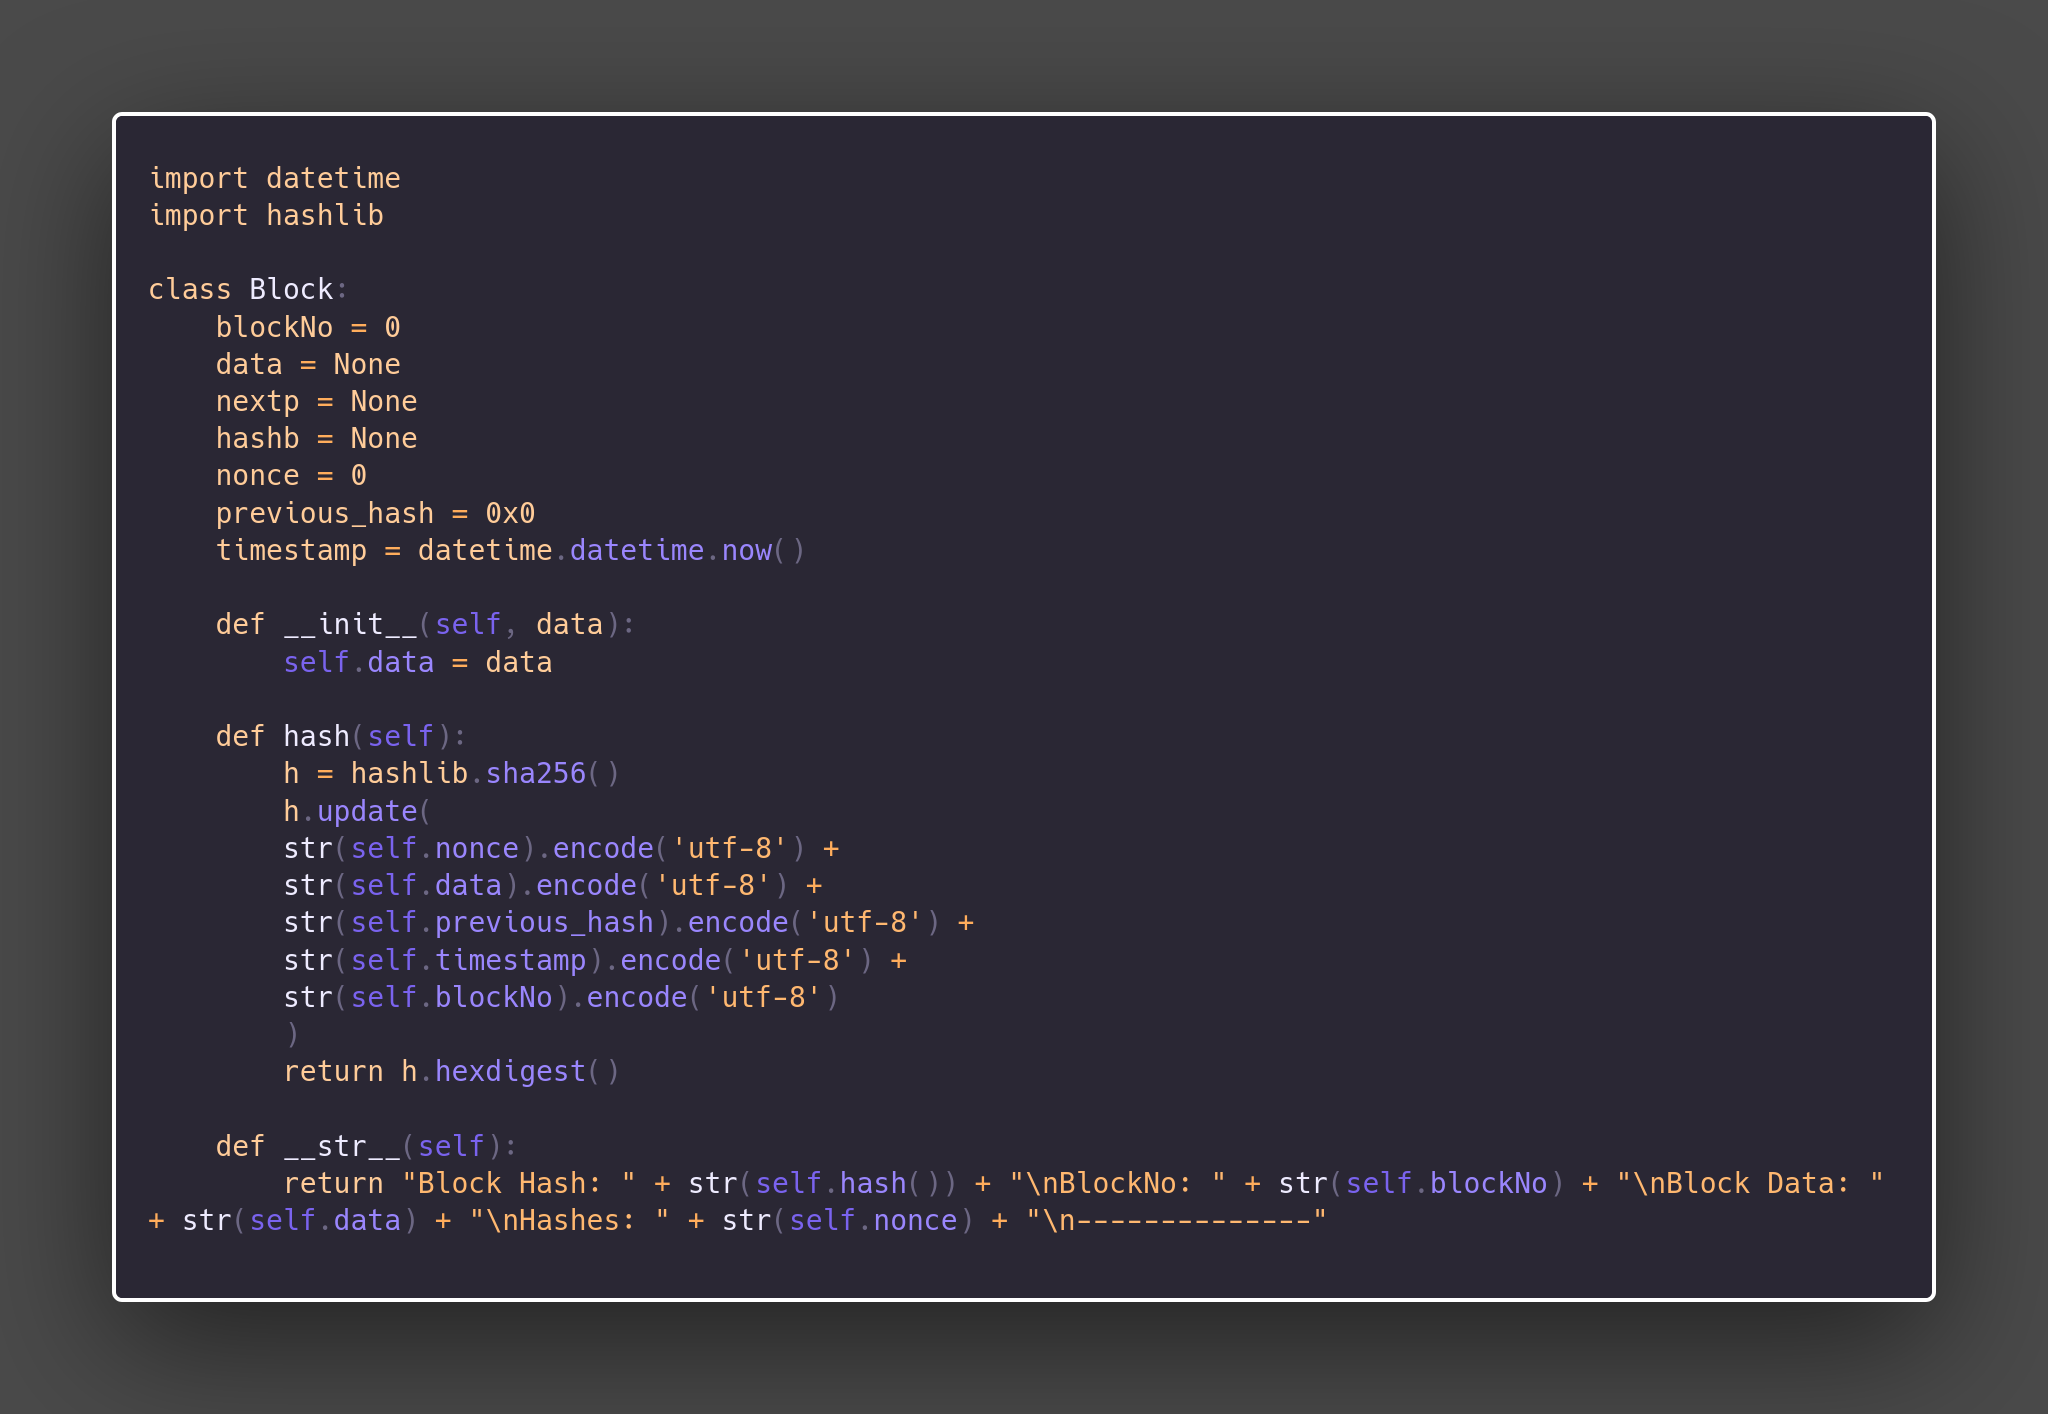
\includegraphics[scale=.17]{carbon.png}    
	\end{frame}
	\begin{frame}{Blockchain}
	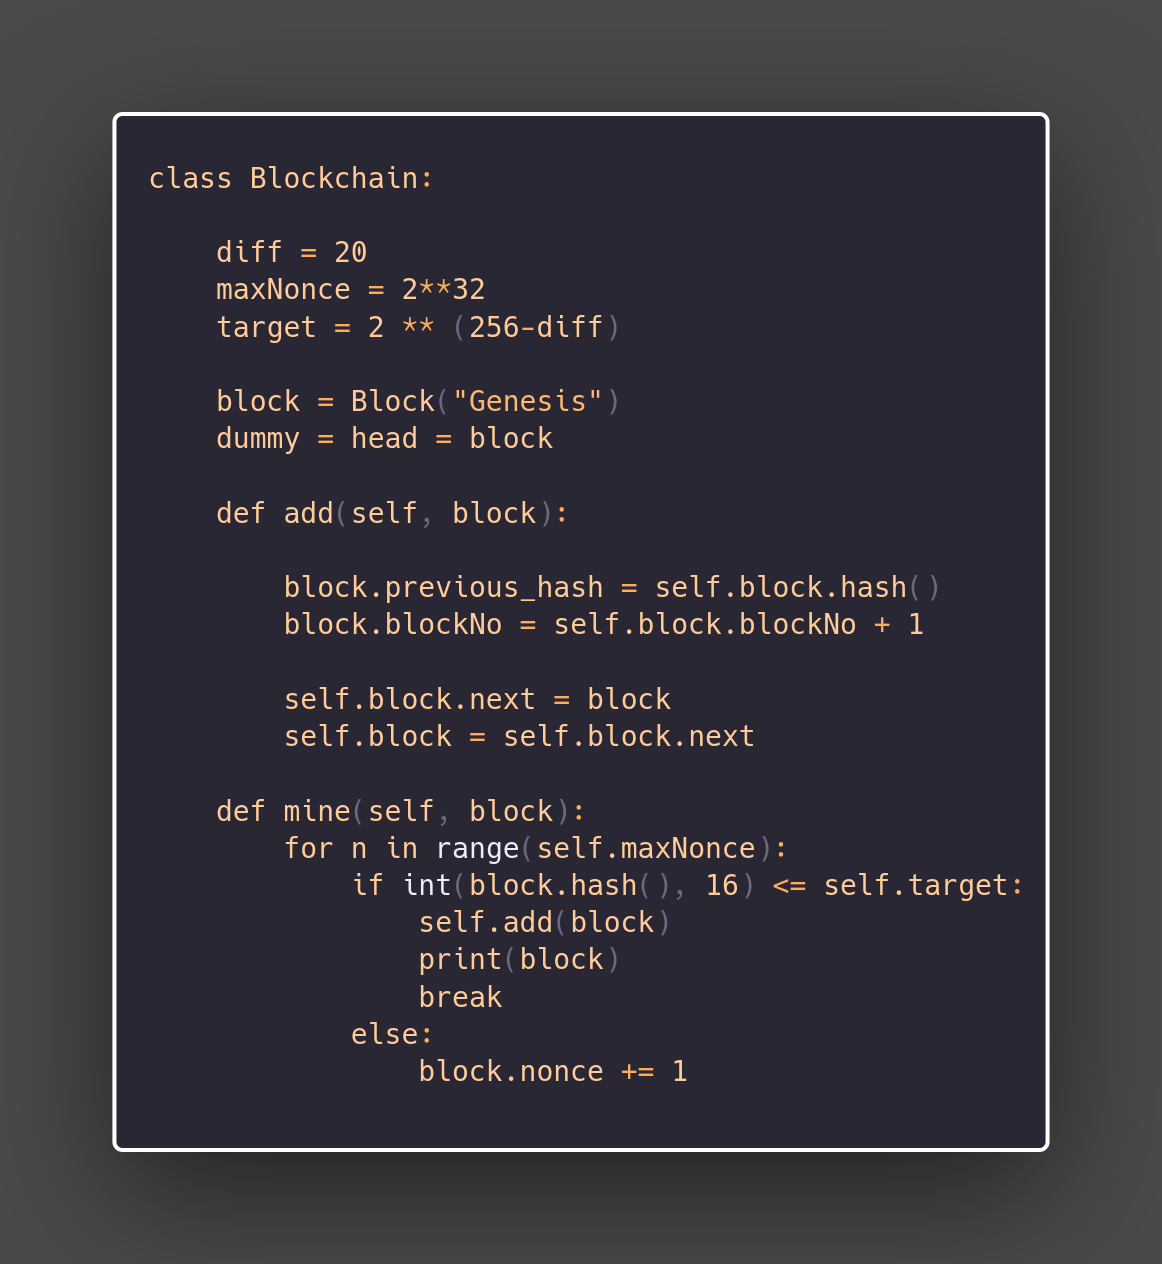
\includegraphics[scale=.17]{2block.png}
	\end{frame}

	\begin{frame}{Output}
		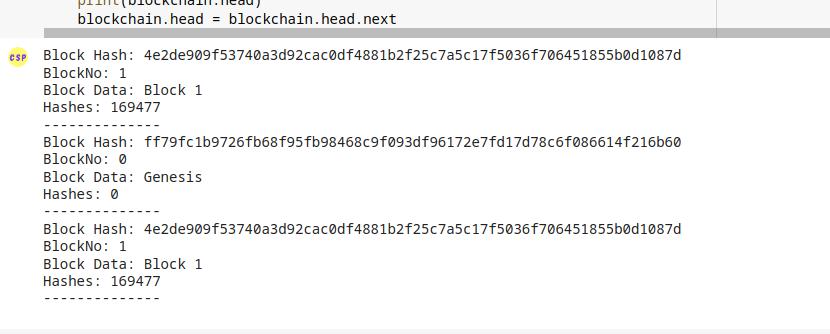
\includegraphics[scale=.8]{out.png}
	\end{frame}

	\section{Cryptography}
	\begin{frame}{Crytography}
		\textbf{Cryptography} is a method of developing techniques and protocols to prevent a third party from accessing and gaining knowledge of the data from the private messages during a communication process. Cryptography is also made up of two ancient Greek terms, Kryptos and Graphein, the former meaning “hidden” and latter being “to write”. 
		\par \textbf{Encryption} It is a process of plaintext (normal text) to a ciphertext (random sequence of bits).
		\par \textbf{Decryption} The inverse process of encryption, conversion of ciphertext to plaintext.
	\end{frame}

	\begin{frame}{Use of Cryptography in Blockchain}
		\normalsize
		Blockchains make use of two types of cryptographic algorithms, asymmetric-key algorithms, and hash functions. 
Hash functions are used to provide the functionality of a single view of blockchain to every participant. 
Blockchains generally use the SHA-256 hashing algorithm as their hash function. 
	\end{frame}

	\begin{frame}{Application of Cryptography}
		\normalsize
		Hashing, public-private key pairs, and the digital signatures together constitute the foundation for the blockchain. 
These cryptographic features make it possible for blocks to get securely linked by other blocks, and also ensure the reliability and immutability of the data stored on the blockchain.
There are a huge number of applications of blockchain technology, and cryptography makes it possible. One of the major real-world applications of cryptography in the blockchain is cryptocurrencies.
	\end{frame}

	\begin{frame}{Cryptography hash function in Blockchain}
		Cryptographic hash functions provide the following benefits to the blockchain:
	\begin{itemize}
		\item \textit{Avalanche effect} – A slight change in the data can result in a significantly different output.
		\item \textit{Uniqueness} – Every input has a unique output.
		\item \textit{Deterministic} – Any input will always have the same output if passed through the hash function.
		\item \textit{Quickness} – The output can be generated in a very small amount of time.
		\item \textit{Reverse engineering is not possible,} i.e. we cannot generate the input by having the output and the hash function.
	\end{itemize}
	\end{frame}

	\begin{frame}{RSA}
		\normalsize
		\textbf{RSA (Rivest–Shamir–Adleman)} is a public-key cryptosystem that is widely used for secure data transmission. It is also one of the oldest. 
		\par
		In a public-key cryptosystem, the encryption key is public and distinct from the decryption key, which is kept secret (private). An RSA user creates and publishes a public key based on two large prime numbers, along with an auxiliary value. The prime numbers are kept secret. Messages can be encrypted by anyone, via the public key, but can only be decoded by someone who knows the prime numbers
	\end{frame}

	\begin{frame}{Code}
		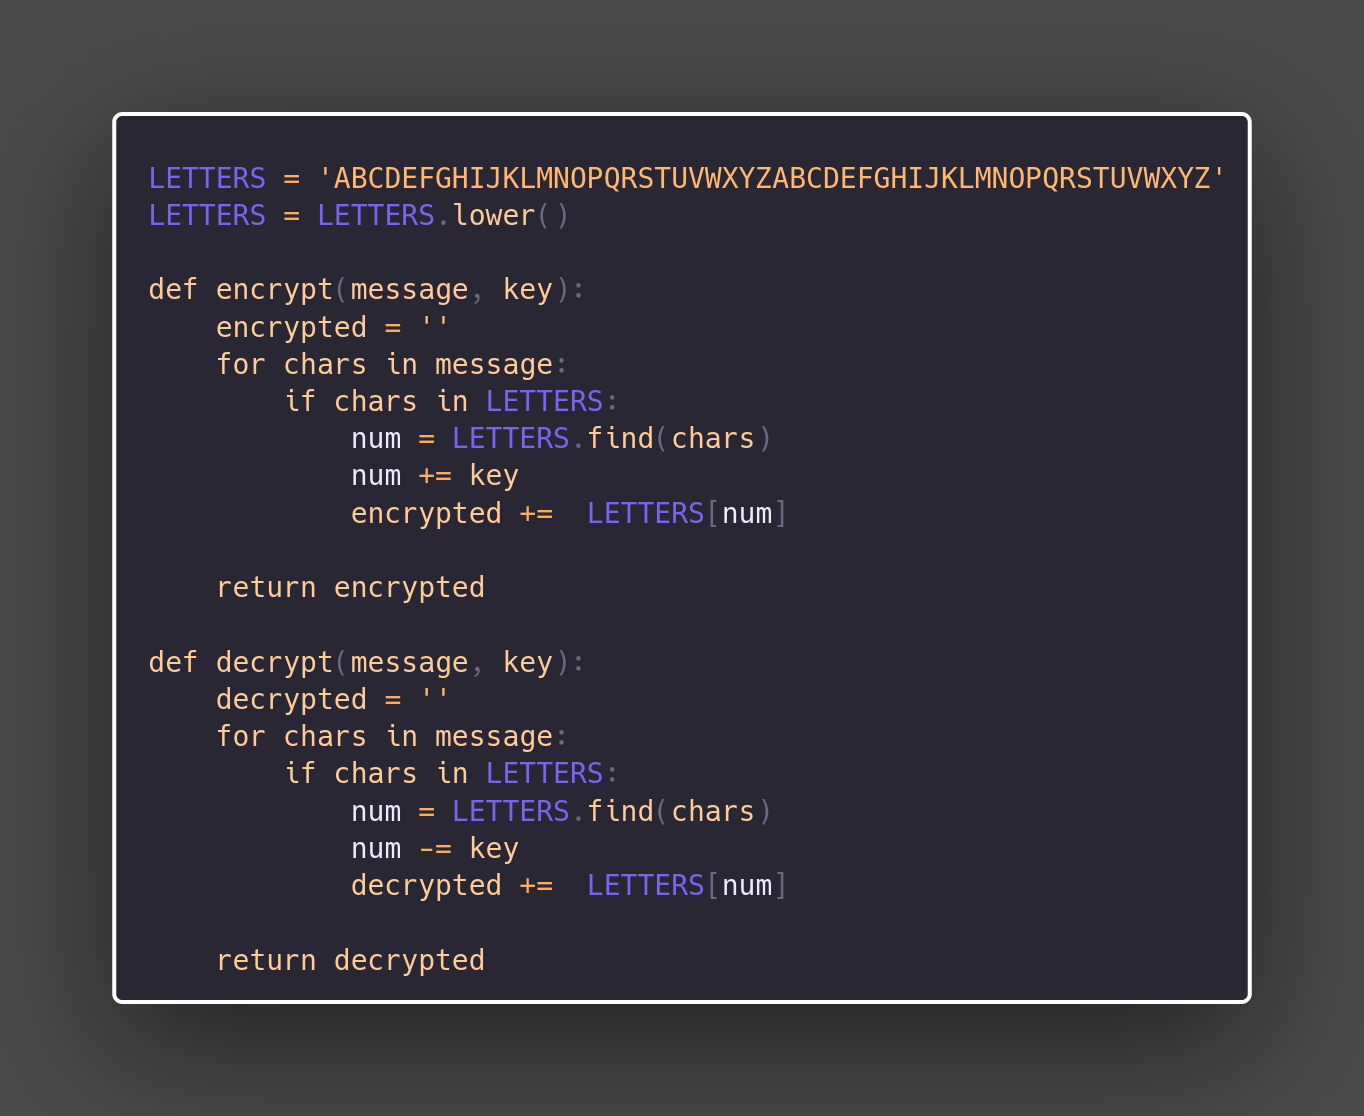
\includegraphics[scale=.17]{3pic.png}
	\end{frame}
	
	\begin{frame}{Output}
		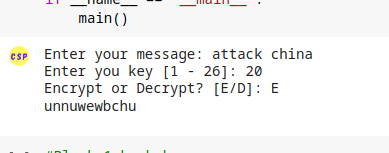
\includegraphics[scale=1]{out2.png}
	\end{frame}
	\begin{frame}
		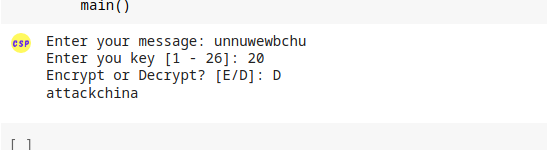
\includegraphics[scale=1]{out3.png}
	\end{frame}
	
	% \section{Remote Procedure Call}
	% \begin{frame}{Remote Procedure Call}
	% 	\normalsize
	% 	In distributed computing, a remote procedure call (RPC) is when a computer program causes a procedure (subroutine) to execute in a different address space (commonly on another computer on a shared network), which is coded as if it were a normal (local) procedure call, without the programmer explicitly coding the details for the remote interaction.
	% 	\par
	% 	RPCs are a form of inter-process communication (IPC), in that different processes have different address spaces: if on the same host machine, they have distinct virtual address spaces, even though the physical address space is the same; while if they are on different hosts, the physical address space is different. Many different (often incompatible) technologies have been used to implement the concept. 
	% \end{frame}

	% \section{Real Time Commnication}
	% \begin{frame}{Real time Communication}
	% 	\normalsize
	% 	Real-time communications (RTC) is any mode of telecommunications in which all users can exchange information instantly or with negligible latency or transmission delays. In this context, the term real-time is synonymous with live.
	% \end{frame}

	\section{References}
	\begin{frame}{References}
	\begin{itemize}
		\item https://www.investopedia.com/terms/b/blockchain.asp
		\item https://www.ibm.com/in-en/topics/what-is-blockchain
		\item https://www.euromoney.com/learning/blockchain-explained/what-is-blockchain
		\item https://en.wikipedia.org/wiki/Blockchain
		\item https://www.pwc.com/us/en/industries/financial-services/fintech/bitcoin-blockchain-cryptocurrency.html
		\item https://builtin.com/blockchain
		\item Nakamoto, Satoshi (October 2008). "Bitcoin: A Peer-to-Peer Electronic Cash System"
	\end{itemize}
	\end{frame}

\end{document}
